\section{Theorie der Dipole in Kristallgittern}
\label{sec:theorie}

Punkte eines Kristallgitters liegen auf einem regelmäßigen drei dimensionalen Raster. Die kleinste Einheit dieser Gitter ist die sogenannte
Elementar- oder Einheitszelle. Die Elementarzelle kann aus einem oder mehreren Punkten bzw. Atomen zusammengesetzt sein.  Die Gitterstruktur
wird durch die gleichmäßige Fortsetzung der Elementarzelle in alle drei Raumrichtungen gebildet. In einem Ionenkristall, wie das welches in
diesem Versuch untersucht wird, wid die Kristallstruktur durch die Ionenbindung zwischen zwei oder mehreren Typen von Ionen gebildet.
Beispielsweise ordnet sich Cäsiumiodid zum einem kubischen innenzentriertem Gitter an. Die Elementarzelle ist in Abbildung \ref{fig:fuckyou}
dargestellt. Die Wechselwirkung zwischen den Gitterpunkten erzeugt ein perdiodisches Potential welches die grundlegenden Eigenschaften, wie
zum Beispiel die Leitfähigkteit, des Festkörpers bestimmt.


\subsection{Dipole durch Leerstellen}

Durch Einbringung eines fremden Ions in den Kristall kann eine Leerstelle entstehen.  Dieser Gitterdefekt ändert zumindest lokal die
Eigenschaften des Kristalls. Das periodische Potential ist gegenüber dem reinen Kristall gestört.  So kann in Cäsiumiodid durch einbau eines
Strontiumions \( Sr^{++} \) eine Leerstelle im Gitter erzeugt werden. Wie in Abbildung \ref{fig:anleitung} dargestellt, bildet sich
ein Dipol zwischen der Leerstelle und dem Strontiumion. Die Dipolachse der Störung zeigt dabei immernoch in richtung einer der Translationsachsen
des Kristalls. Die Ausrichtung des Dipols kann sich durch sogenannte Leerstellendiffusion ändern. Dafür muss Arbeit aufgebracht werden um das
Gitterpotential an der Stelle zu überwinden. Die thermische Energieverteilung der Dipole ist durch die Boltzmannstatistik nach Gleichung
\ref{eq:boltzmann} vorgegeben. Dabei ist $W$ die erforderliche Energie die die Leerstelle benötigt um die Gitterstelle zu wechseln. $T$ ist
die Temperatur und $k_B = \SI{1,38064852E-23}{\joule \per \kelvin}$ die Boltzmannkonstante.

\begin{equation}
  \label{eq:boltzmann}
  E_D \propto e^{- \frac{W}{k_B T}}
\end{equation}

Die Relaxationszeit, die Zeit nach der die Dipole ihre Orientierung wechseln beträgt im Mittel

\begin{equation}
  \label{eq:time}
  \tau(T) = \tau_0 e^{ \frac{W}{k_B T}}.
\end{equation}

Ziel dieses Versuches wird sein die Aktivierungsenergie $W$ und die charackteristische Relaxationszeit $\tau_0$ zu bestimmen.

\subsection{Dipole im äußeren elektrischen Feld }

Wird das dotierte Gitter einem elektrischen Feld ausgesetzt, so werden sich die Dipole, soweit wie es die Gitterstruktur zulässt, in Feldlinienrichtung
ausrichten. Durch thermische Energie wird jedoch zu jeder Zeit ein Teil der Dipole die Ausrichtung ändern. Der Anteil der in Feldrichtung
ausgerichteten Dipole ist also stochastisch bestimmt. Das ist die Grundlage für die Anwendbarkeit der Langevin Formel \ref{eq:langevin}.
Diese beschreibt ursprünglich die Magnetisierung eines Paramagnetischen Materials unter Einfluss eines äußeren Magnetfelds. Die Langevin Formel ist die klassische
Näherung der Brillouin Formel \ref{eq:brillouin}.
Dabei ist $x = \frac{\vec{m}_B \vec{B}}{k_B T}$ mit dem äußeren Magnetfeld $\vec{B}$ und dem magnetischen
Dipolmoment $\vec{m}_B$. Analog ist im Fall äußerer elektrische Felder, wie in diesem Versuch,   $x = \frac{\vec{m} \vec{E}}{k_B T}$ mit dem elektrischen Dipolmoment
$\vec{m}$ und dem externen elektrischen Feld $\vec{E}$. Bei richtiger Ausrichtung der elektrischen Feldlinien zu den Gittervektoren des Kristalls
ist die Richtung des Dipolmoments im Mittel paralell zum elektrischen Feld. Dann lässt sich die Langevin Funktion parametrisieren mit
$x= \frac{m E}{k_B T}$. Der Verlauf der Langevin Funktion ist in Abbildung \ref{fig:langevin} skizziert.

\begin{equation}
  \label{eq:brillouin}
  B_J(x) = \frac{2J + 1}{2J} \coth \left ( \frac{2J + 1}{2J} x \right ) - \frac{1}{2J} \coth \left ( \frac{1}{2J} x \right )
\end{equation}

\begin{equation}
  \label{eq:langevin}
  L(x) = \coth(x) - \frac{1}{x}
\end{equation}

\begin{figure}
  \label{fig:langevin}
  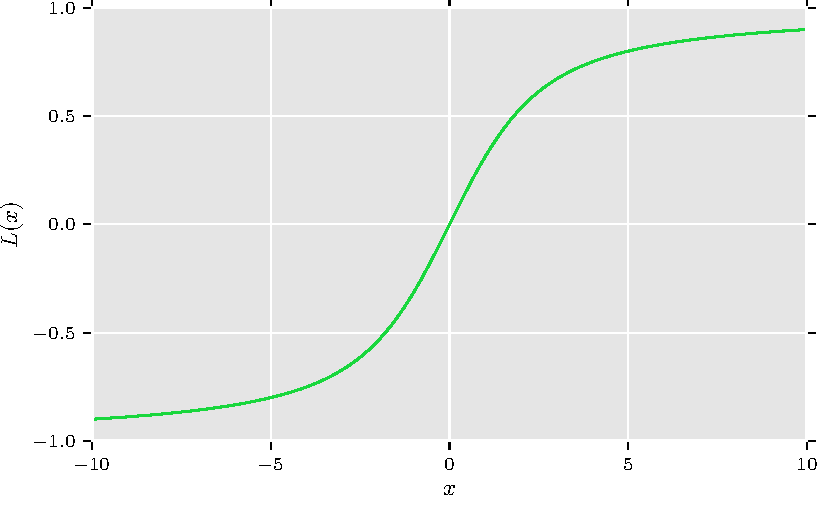
\includegraphics{./plots/langevin.pdf}
  \caption{Langevin Funktion im Bereich von -10 bis 10.}
\end{figure}


Im folgenden Versuchsaufbau ist $ x << 1 $ wodurch die Näherung $L(x) \approx \frac{x}{3}$ genutzt werden kann. Somit ergibt sich für den Anteil der zur Feldrichtung
ausgerichteten Dipole

\begin{equation}
  \label{eq:dipoles}
  L(T) \approx \frac{m E}{3 k_B T}.
\end{equation}
